% called by main.tex
%
\chapter{Resultados}
\label{ch::chapter4}

En este capitulo se presentaran los resultados obtenidos durante las campañas de expermientos, cuyo 
objetivo es el de evaluar el impacto de la integración de HQC sobre una red IoT formada por sistemas 
embebidos. 

El analisis se basa en estudiar el comportamiento del sistema bajo diferentes condiciones experimentales
como se reviso en el capitulo anterior. Los resultados estan organizados por topologías, comenzando 
con la configuración P2P, y continuando con Árbol, Linea y Estrella. Finalmente se realiza una 
comparación global entre las diferentes topologías, con el proposito de identificar las principales 
diferencias observadas. 

Para obtener los datos, se realizaron 3 pruebas por condición, y se realizo una media ponderada para cada
condición de cada topologia.

\section{P2P}
Para comenzar con la campaña de pruebas, se ejecutaron las condiciones de prueba 0, 2 y 4 sobre 
la topología P2P, en la que se busca conocer el impacto de transportar HQC entre dos nodos, o nodo y servidor.

\begin{figure}[htbp]
    \centering
    % Primera fila
    \begin{subfigure}[b]{0.48\textwidth}
        \centering
        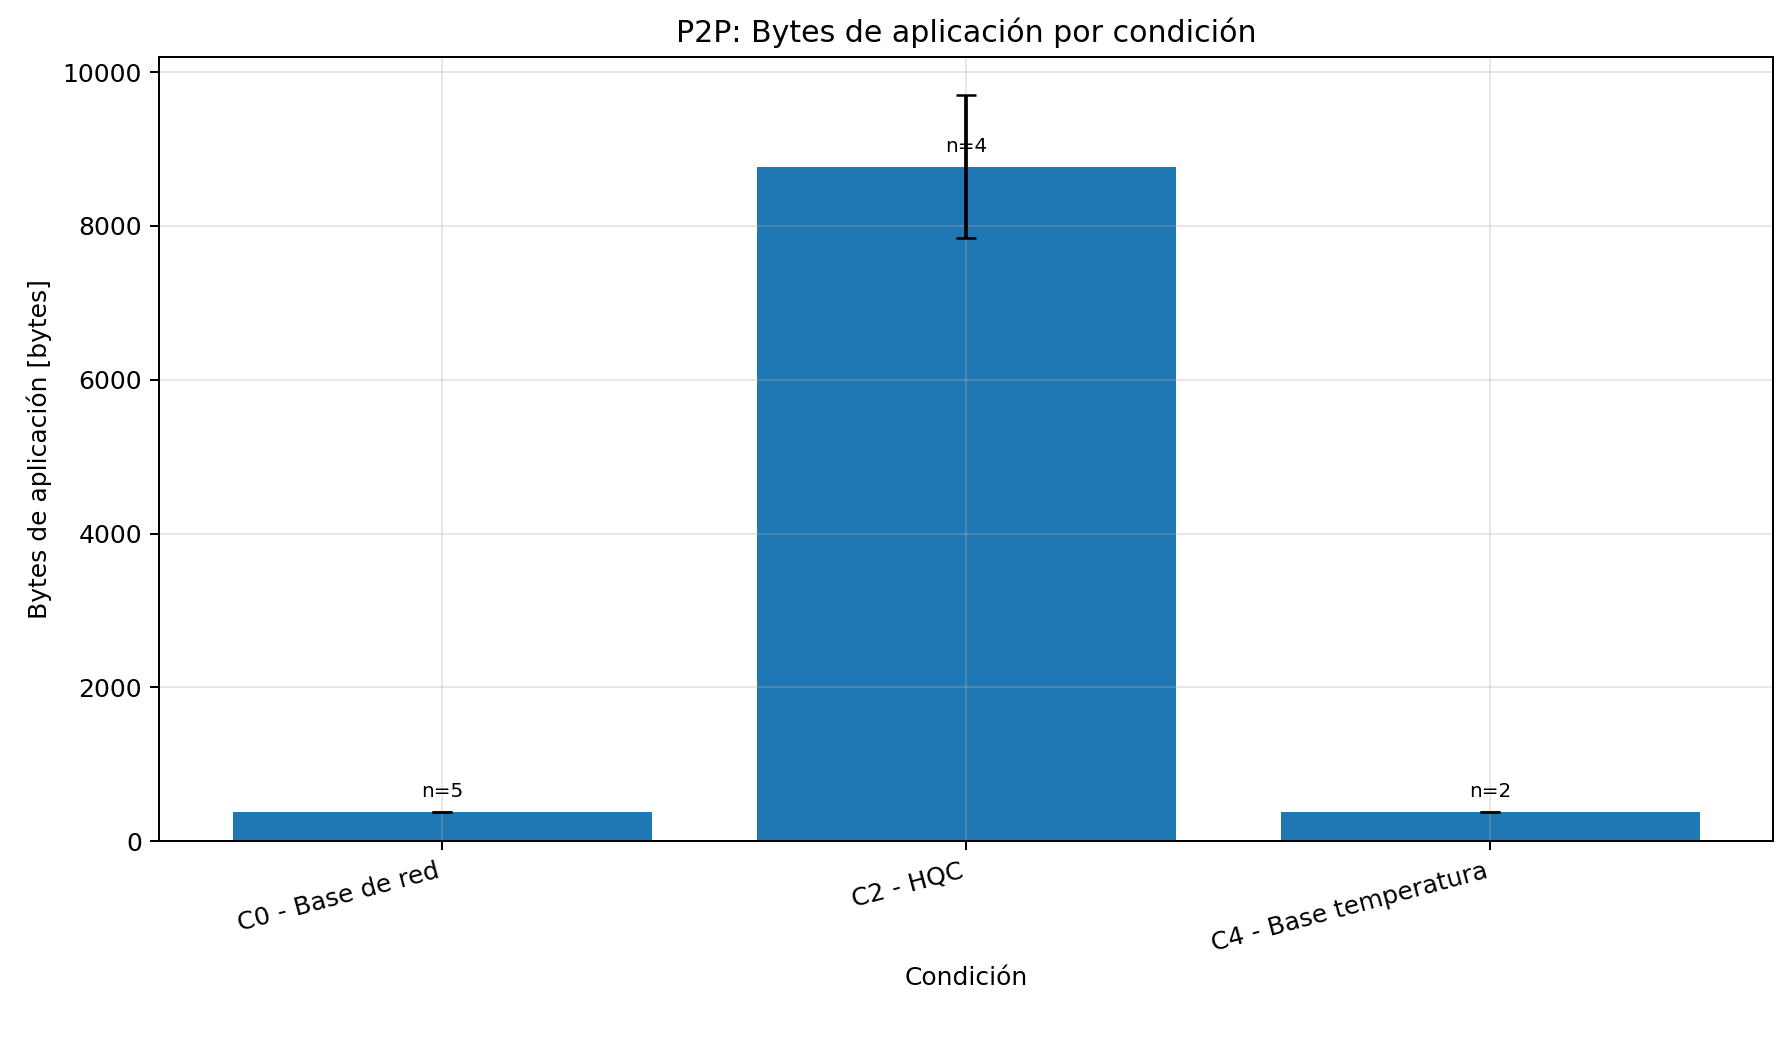
\includegraphics[width=\textwidth]{figures/Imagenes/Graficas_HQC/P2P/P2P_app_bytes_por_condicion.png}
        \caption{Bytes de la app}
        \label{fig:bytes_por_condicion}
    \end{subfigure}
    \hfill % Espacio horizontal entre columnas
    \begin{subfigure}[b]{0.48\textwidth}
        \centering
        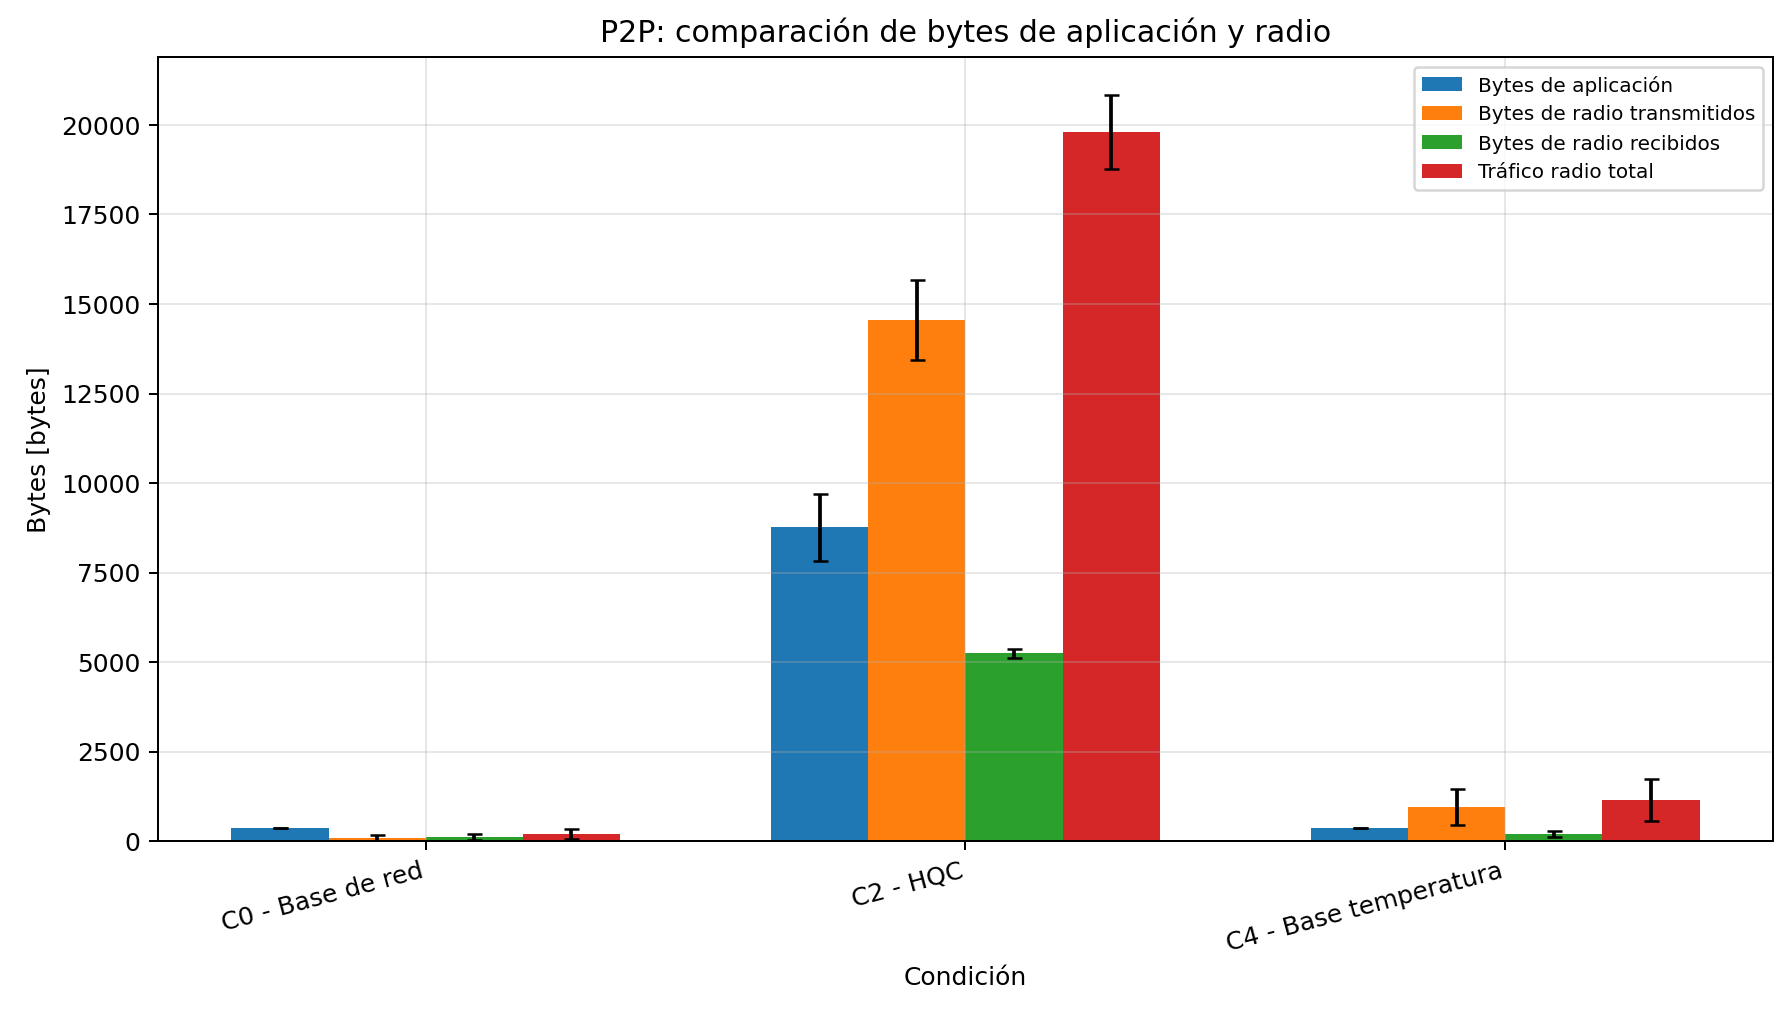
\includegraphics[width=\textwidth]{figures/Imagenes/Graficas_HQC/P2P/P2P_comparacion_app_tx_rx_total.png}
        \caption{Comparación tx rx}
        \label{fig:comparacion}
    \end{subfigure}

    \vspace{0.5cm} % Espacio vertical entre filas

    \begin{subfigure}[b]{0.48\textwidth}
        \centering
        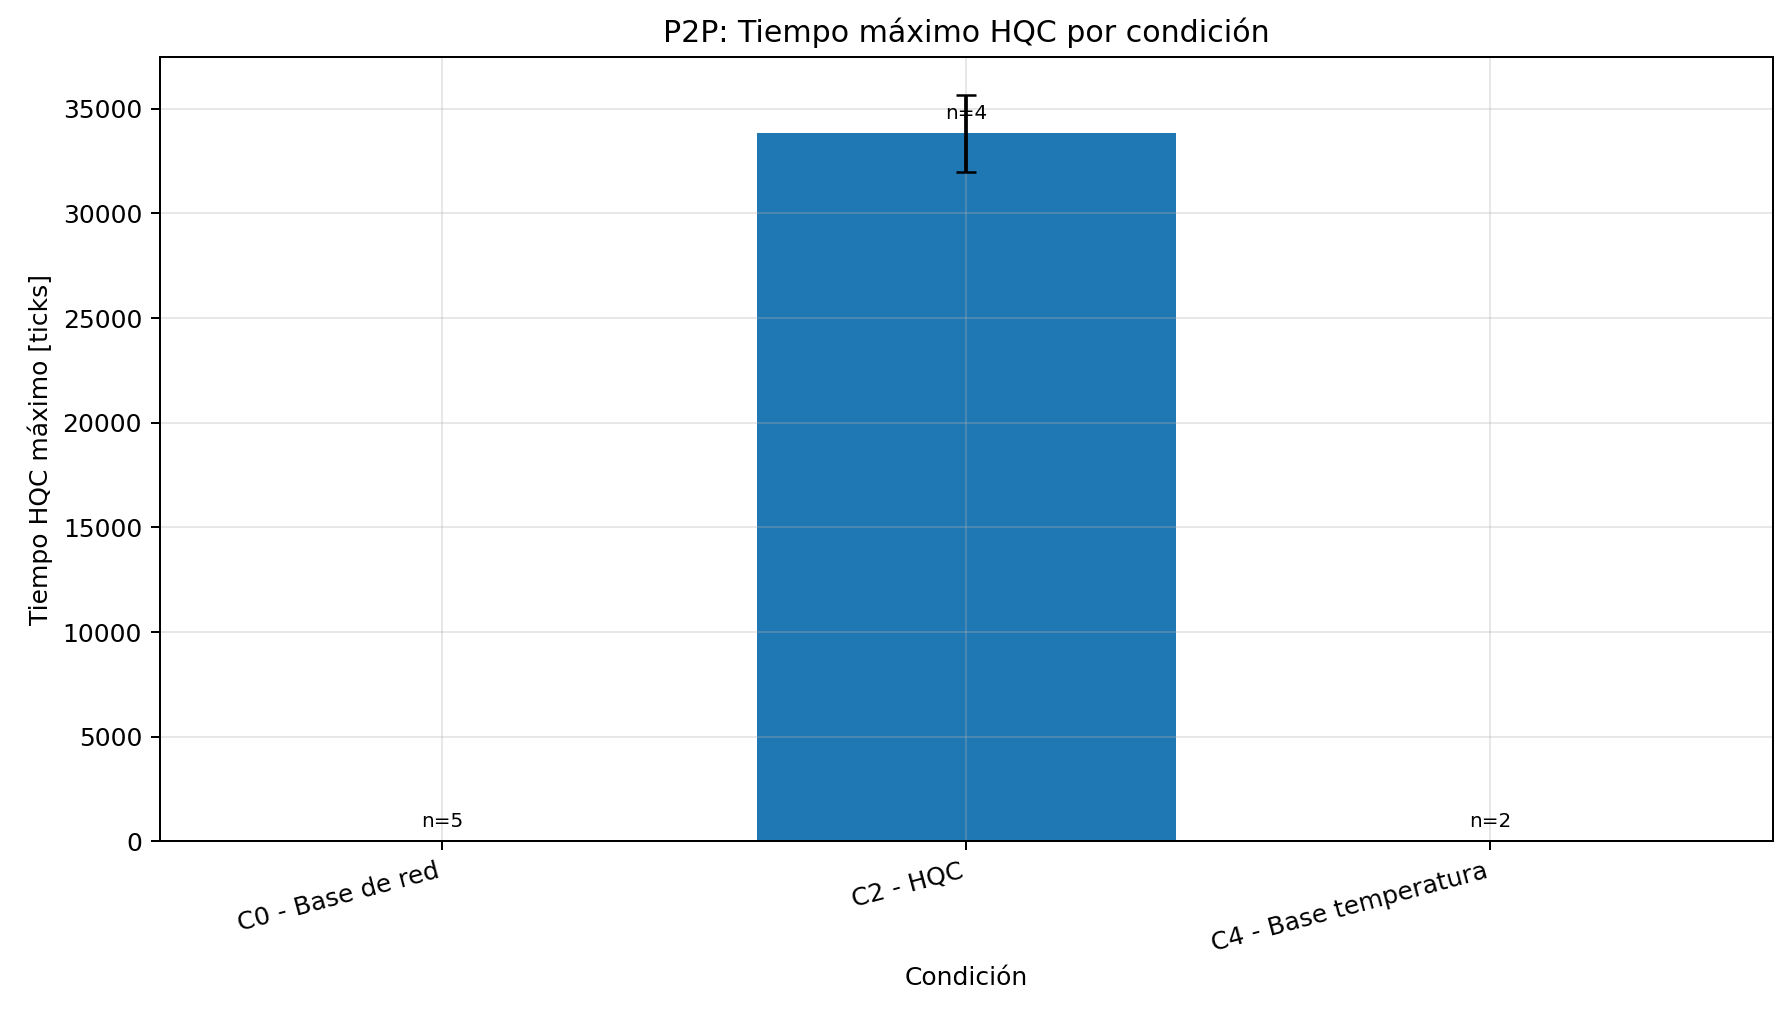
\includegraphics[width=\textwidth]{figures/Imagenes/Graficas_HQC/P2P/P2P_hqc_total_ticks_max_por_condicion.png}
        \caption{Tiempo HQC}
        \label{fig:Tiempo_hqc}
    \end{subfigure}

    % Título general de la matriz
    \caption{Análisis global del tráfico generado en escenarios P2P}
    \label{fig:matriz_p2p_global} % Etiqueta principal de todo el bloque
    
\end{figure}

En la Figura~\ref{fig:bytes_por_condicion} se puede observar como, en la condición 2 se genera un tráfico 
masivo, alcanzando los 8KB en promedio. Esto significa que el transporte de las claves publica y privada 
son en mayor medida el gran cuello de botella de el protocolo. A diferencia de la condición 4, en la que 
el cifrado de los datos a penas afecta al tráfico entre los nodos. 

La Figura~\ref{fig:comparacion} muestra una capa nueva, durante el establecimiento de la red segura con HQC, 
se registraron 8KB aproximadamente, mientras que los contadores de radio registraron 14KB transmitidos. La diferencia
puede atribuirse tanto al efecto de la sobercarga en las comunicaciones, y a las posibles retransmisiones, aunque 
no ha sido posible cuantificar individualmente estas contribuciones. 

Por otro lado, tenemos un tiempo medio de 33000 Ticks aproximadamente en establecer la red segura, asi como el procesamiento
matematico de la cpu, según nos marca la Figura~\ref{fig:Tiempo_hqc}. Este comportamiento es el esperado, debido al tamaño de las claves transportadas.

\section{Estrella}

El siguiente paso es realizar la campaña de pruebas, se ejecutan las las condiciones de pruebas 0, 2, 3 y 4 sobre la topología estrella, las primeras
tres figuras generadas con las siguientes. 

\begin{figure}[htbp]
    \centering
    % Primera fila
    \begin{subfigure}[b]{0.495\textwidth}
        \centering
        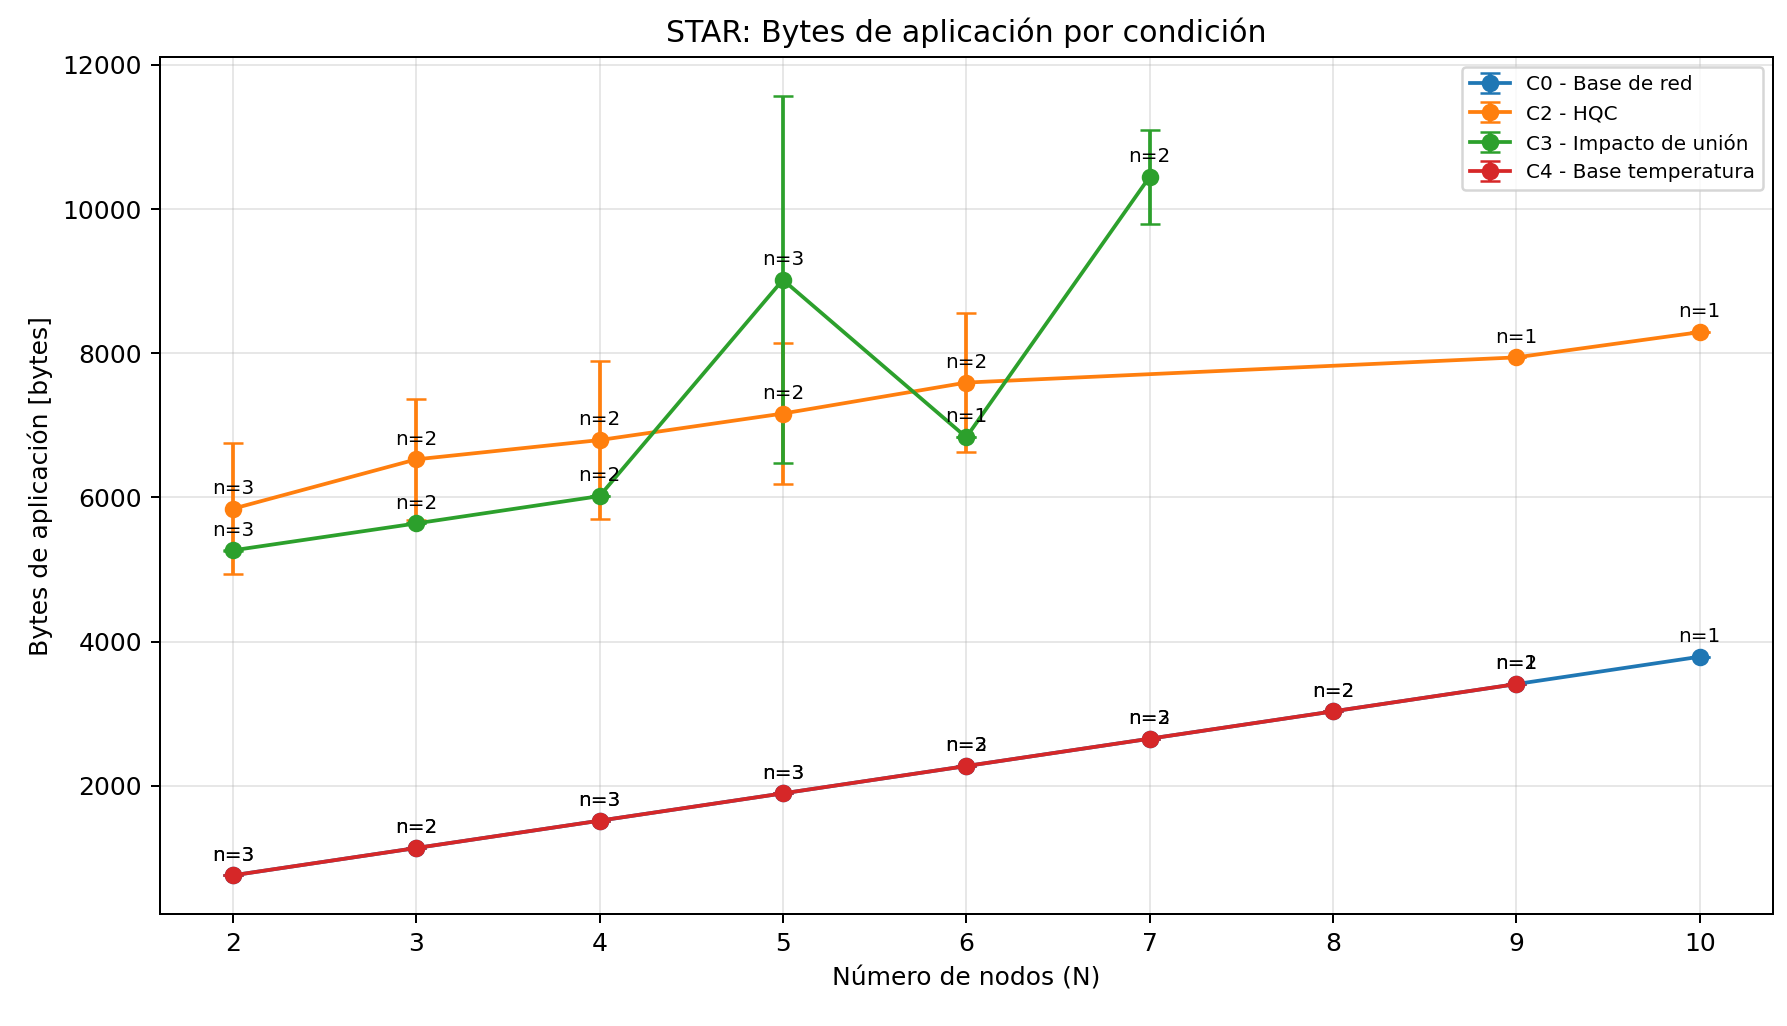
\includegraphics[width=\textwidth]{figures/Imagenes/Graficas_HQC/STAR/STAR_app_bytes_por_condicion.png}
        \caption{Bytes de la app}
        \label{fig:bytes_por_condicion_star}
    \end{subfigure}
    \hfill % Espacio horizontal entre columnas
    \begin{subfigure}[b]{0.495\textwidth}
        \centering
        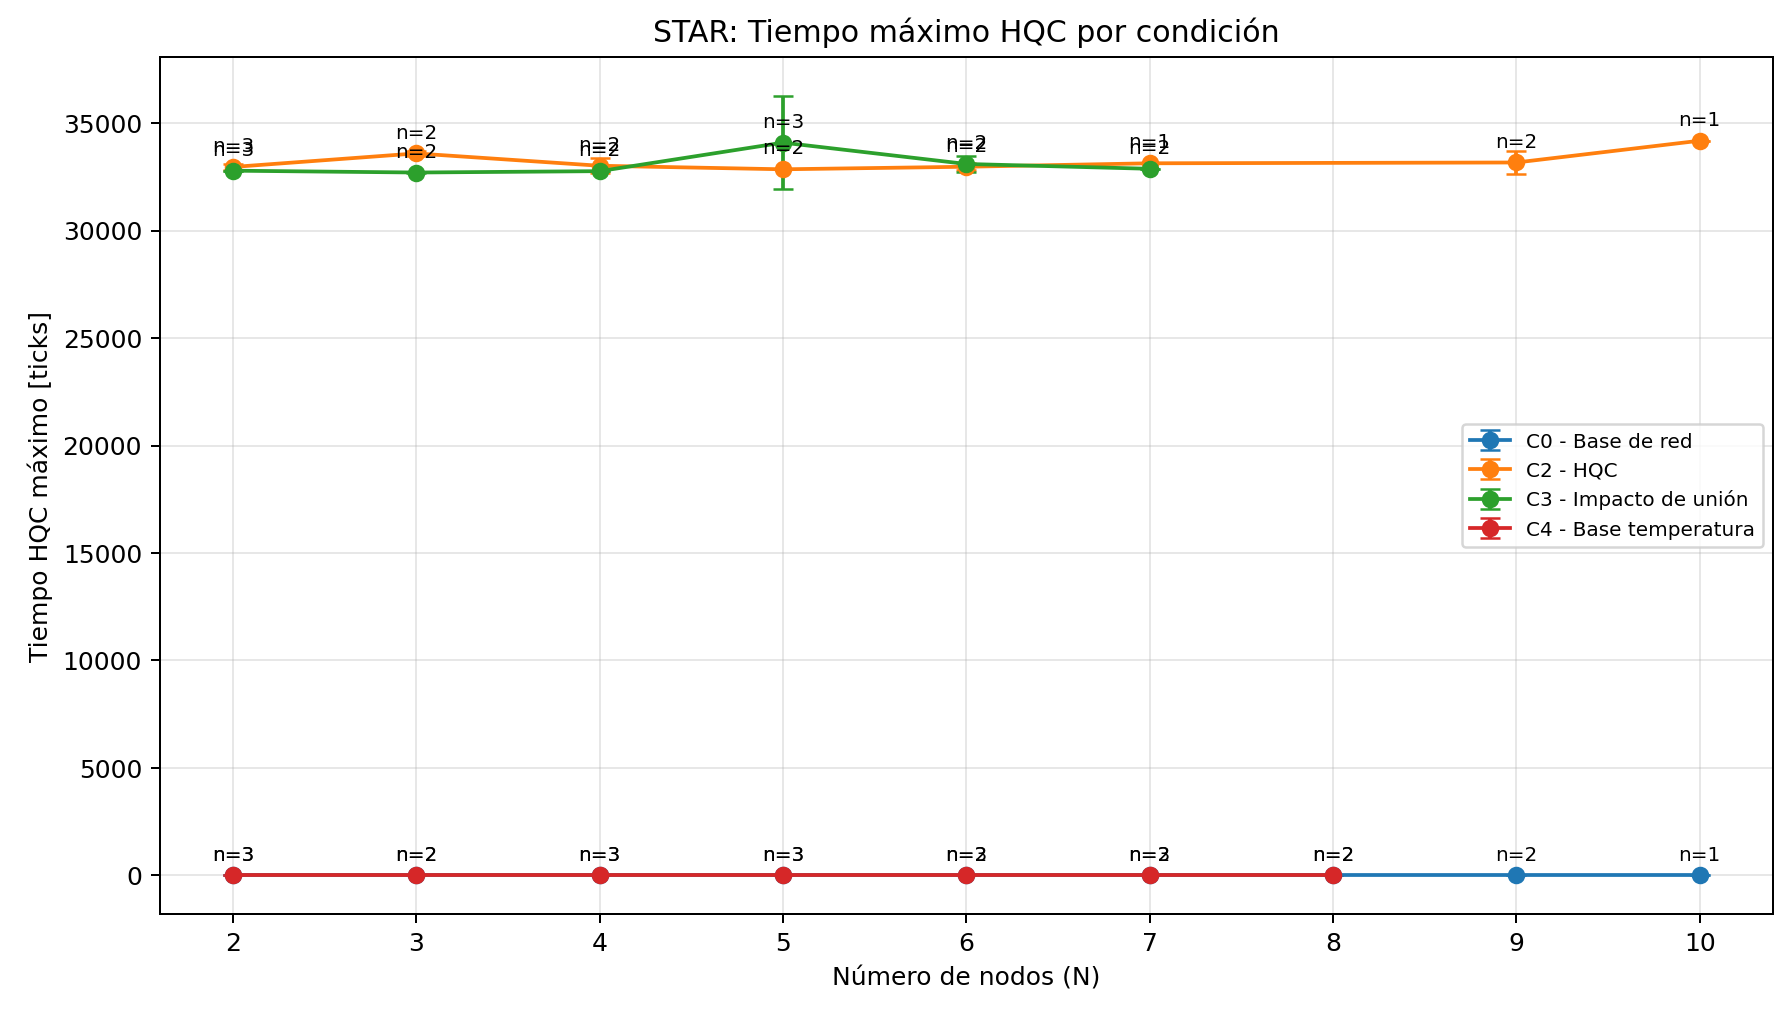
\includegraphics[width=\textwidth]{figures/Imagenes/Graficas_HQC/STAR/STAR_hqc_total_ticks_max_por_condicion.png}
        \caption{Tiempos totales por condición}
        \label{fig:tiempo_star}
    \end{subfigure}

    \vspace{0.5cm} % Espacio vertical entre filas

    \begin{subfigure}[b]{0.51\textwidth}
        \centering
        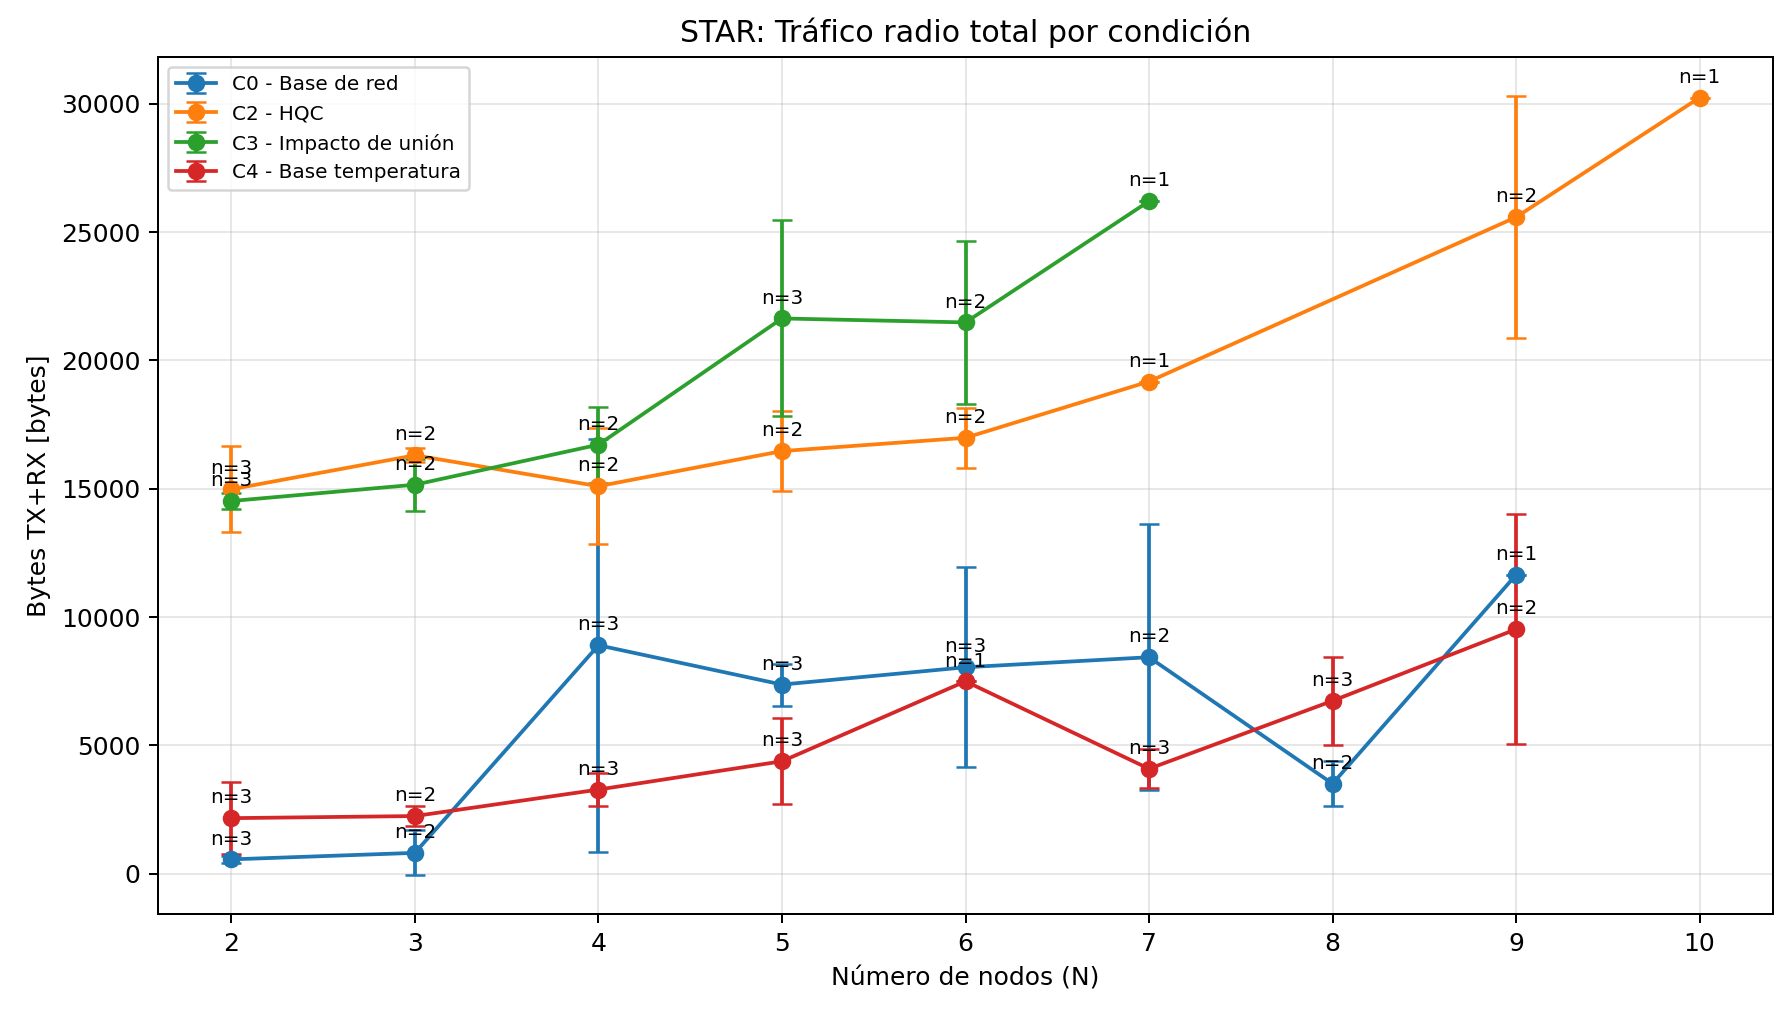
\includegraphics[width=\textwidth]{figures/Imagenes/Graficas_HQC/STAR/STAR_radio_bytes_por_condicion.png}
        \caption{Tráfico total por condición}
        \label{fig:trafico_star}
    \end{subfigure}

    % Título general de la matriz
    \caption{Análisis global del tráfico generado en escenarios star}
    \label{fig:matriz_star_global} % Etiqueta principal de todo el bloque
    
\end{figure}

Como se puede observar en la Figura~\ref{fig:bytes_por_condicion_star}, las condiciones 0 y 4 tienen un comportamiento lineal, 
creciendo a medida que crece la red, es normal esperar este comportamiento, debido a que crece la dificultad de mantener la 
red con el crecimiento de la misma. Con respecto a la condicion 2, se tiene un comienzo relativamente alto, al tener 2 nodos 
sin contar con el servidor, y esperable debido a que no existen saltos intermedios, sin embargo, al crecer la red, crece con 
una pendiente menor que la condición 4. 

Existen anomalias en la condición 3, teniendo en cuenta que en esta condición se pretende estudiar el impacto que tiene la unión 
en una red establecida junto con trafico de datos cifrados, con una cantidad pequeña de nodos tiene un comportamiento similar 
a la condición 2, lo que representa un comportamiento normal, debido a que los canales de comunicación estan despejados. A partir
del 5 nodo, existe una saturación del canal, por lo que el servidor tiene que gestionar las comunicacione existentes mientras procesa
la unión del nuevo nodo y sus datos. 

Los tiempos de establecimiento de la comunicación segura son estables durante todas las condiciones y numero de nodos, como muesta 
la Figura~\ref{fig:tiempo_star}, como es de esperar, al no tener saltos intermedios, no existe penalización de retransmisión entre nodos.

Por otro lado, es importante mencionar el tráfico de radio total de la Figura~\ref{fig:trafico_star}, donde se observa que el tráfico 
en la condición 3 para 5 nodos se dispara a más de 20KB aproximadamente, demostrando que el tráfico de radio en esta condición
támbien se debe a retransmisiones y paquetes de control. Al añadir un nodo extra, junto con los datos cifrados, el medio físico 
se congestiona, provocando que el protocolo deba reenviar paquetes. 

El crecimiento eponencial de la condición C2, revelando el coste en escalabilidad de HQC en una topología estrella. Aunque el protocolo
intente mantener un flujo controlado, el servidor sufre un desgaste en el uso de la radio. 

\begin{figure}
    
    \centering
    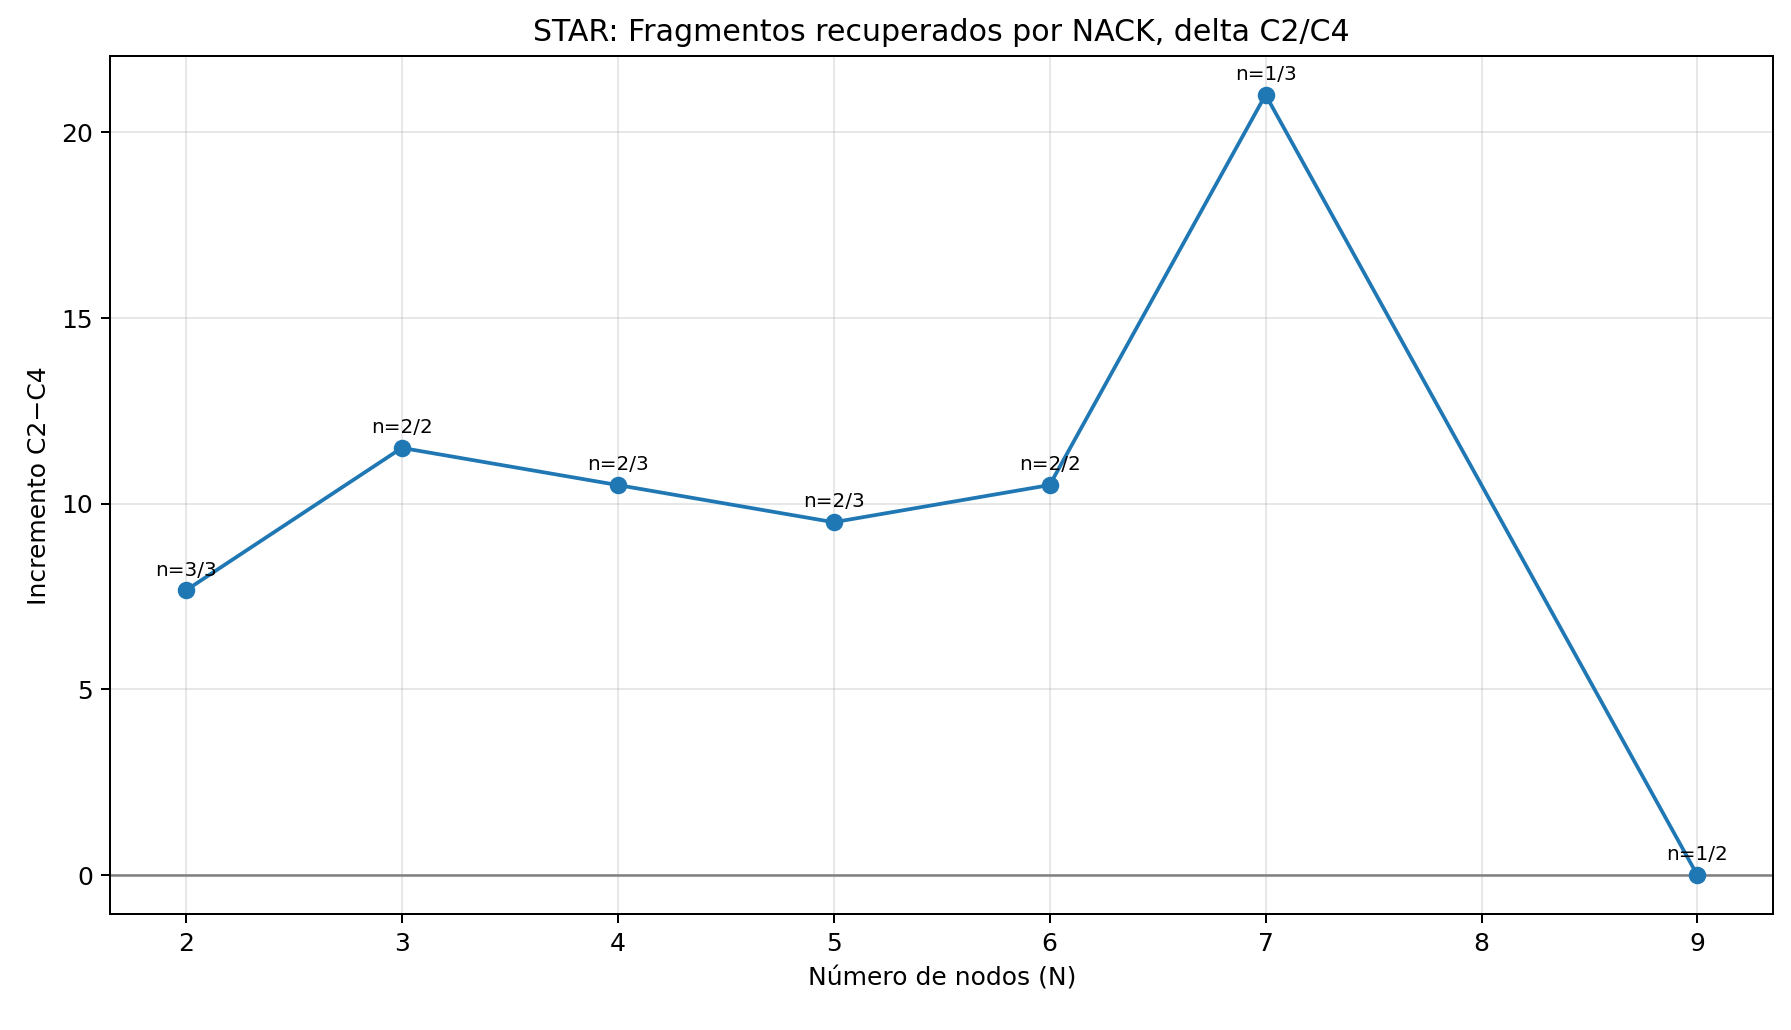
\includegraphics[width=\textwidth]{figures/Imagenes/Graficas_HQC/STAR/STAR_nack_retransmitted_fragments_C2_menos_C4.png}
    \caption{Fragmentos recuperados NACK}
    \label{fig:NACK_STAR}

\end{figure}

Para terminar de completar la imagen de la topología estrella, la Figura~\ref{fig:NACK_STAR}, demuestra el $\delta C_2/C_4$ en fragmentos recuperados
por el NACK. Los resultados revelan una correlación con las metricas de trafico: al alcanzar los 7 nodos, el sistema sufre un pico crítico de más de 
21 fragmentos perdidos y recuperados por NACK. Esto demuestra que el tamaño de las claves del algoritmo HQC satura el medio físico de la topología, 
provocando colisiones masivas y forzando al protocolo a realizar retransmisiones. El escenario de 9 nodos y su desplome denota una situación de saturación 
donde la congestion impide la correcta señalización de paquetes perdidos.

\section{Linea}


\section{Ábol}

